
\subsection{2.8. Симметрия молекул. Элементы и операции симметрии. Символика Шёнфлиса.} 

\par\bigskip
	
\textbf{Симметрия молекул - совокупность операций симметрии,
	применение которых переводит молекулу в физически
	тождественный объект, то есть, саму в себя.} Симметрия молекул
играет фундаментальную роль в молекулярной спектроскопии,
позволяет проводить классификацию уровней энергии молекул. С
помощью аппарата симметрии появляется возможность строить
диаграммы молекулярных орбиталей: если у какой-либо орбитали
нет пары по симметрии, то она выступит как несвязывающая;
перекрываются только орбитали одинаковой симметрии.

\par\smallskip

Математическая операция или превращение, приводящее к той же
самой фигуре, что и исходная, или к её зеркальному отображению
называется операцией симметрии. Такие операции включают
отражение, вращение и трансляцию (смещение в другое
положение). Набор всех операций, оставляющих фигуру
неизменной, называется группой симметрии для данной фигуры.
Таким образом, операции симметрии составляют группу
симметрии.

\par\smallskip

Элементы симметрии не являются элементами групп симметрии.
Каждому элементу отвечает замкнутый набор операции симметрии,
то есть, элемент симметрии может иметь более одной операции
симметрии, связанной с ним.

\begin{center}
\textbf{Рассмотрим основные элементы симметрии и связанные с ними
	операции:}
\end{center}

1) \textbf{Идентичность (тождественность)}

\par\smallskip

Обозначается Е

\par\smallskip

Такой элемент симметрии есть во всех объектах. Он
соответствует такой операции, что с объектом ничего не
происходит (тождественное преобразование)

\par\smallskip

2) \textbf{Инверсия} 

\par\smallskip

Обозначается i

\par\smallskip

В результате операции, соответствующей элементу «инверсия»,
все атомы отражаются через центр молекулы:

$$R(x,y,z) \longrightarrow -R(-x,-y,-z)$$

3) \textbf{Поворотная ось}

\par\smallskip

Обозначается $C_n$

\par\smallskip

$n=\frac{360^\circ}{\alpha}$, где $\alpha$ - угол поворота, а $n$ - порядок поворотной оси.

\par\smallskip

Поворот вокруг оси, проходящей через молекулу. В
высокосимметричных точечных группах их может быть несколько.
Если она одна, по ней обычно выбирают ось $z$.

\par\smallskip

Каждой оси симметрии соответстуют свои операции симметрии.
Так, к примеру, у оси $C_3$ есть две операции симметрии:

\par\smallskip

$C_3^1$ - поворот на $120^\circ$; $C_3^2$ - поворот на $240^\circ$. !Но: нет   $C_3^3$, т.к. это E.

\par\smallskip

И у оси $C_4$тоже двe:

\par\smallskip

$C_4^1$ - поворот на $90^\circ$.  $C_4^2$ - нет, т.к. это равносильно $C_2^1$. $C_4^3$ - поворот на $270^\circ$. $C_4^4$ - нет, т.к. это E.

\par\smallskip

Ясно, что $C_n^k = C_n^{k-n}$ (например, $C_4^3 = C_4^{-1}$, т.к. поворот вокруг оси 4-го порядка на $270^\circ$ в одну сторону эквивалентен повороту на $90^\circ$ вокруг той же оси в другую сторону).

\par\smallskip
	
4) \textbf{Зеркальная плоскость}

\par\smallskip

Обозначается $\sigma$

\par\smallskip

Отражение всех атомов в плоскости, проходящей через
молекулу.

\par\smallskip
Различают вертикальные, горизонтальные и диэдрические
зеркальные плоскости.

\par\smallskip

5) \textbf{Зеркально-поворотная ось}

\par\smallskip 

Обозначается $S_n$

\par\smallskip

Этот элемент симметрии является комбинацией поворотной
оси и отражения в плоскости, перпендикулярной данной оси.

\par\smallskip

$S_2$ нет, поскольку это эквивалентно операции инверсии:

\begin{figure}[H]
	\centering
	{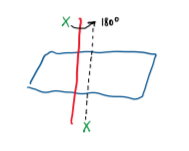
\includegraphics[scale=1.5]{28.png}}
\end{figure}

Из $S_{2n}$ следует наличие $C_n$.

\par\smallskip

	
Число операций следует из числа операций для $C_n$ (если есть
плоскость отражения):

\par\smallskip

Например, для $S_4$ есть $S_4^1$ (поворот на $90^\circ$ + отражение)	и $S_4^3$ (поворот на $270^\circ$ + отрожение).

\begin{center}
\textbf{Символика Шёнфлиса.}
\end{center}	

Символы Шёнфлиса - одно из обозначений точечных групп
симметрии.

\par\smallskip

С - одна главная поворотная ось, нет зеркально-поворотных осей,
нет побочных осей второго порядка.

\par\smallskip


S - одна зеркально-поворотная ось, соответствующая оси высшего
порядка, нет побочных осей второго порядка.

\par\smallskip

D - одна зеркально-поворотная ось, соответствующая ей ось
высшего порядка, есть побочные оси второго порядка,
перпендикулярные главной оси.

\par\smallskip


T, O, I - обозначения для групп, где несколько осей высшего
порядка (тетраэдр, октаэдр (куб), икосаэдр (додекаэдр)). 

\par\smallskip	
	
Цифровой индекс - порядок поворотной оси (в группах S -
порядок зеркально-поворотной оси).

\par\smallskip

Буквенные индексы:	

\par\smallskip

v - есть вертикальные плоскости.

\par\smallskip

d - диэдрические плоскости (чередуются с побочными $C_2 \perp C_n$).

\par\smallskip

h - горизонтальная плоскость.

\par\smallskip
	
Предельные группы для линейных систем:

\par\smallskip

$C_{\infty v}$ (нет $\sigma _h$) и  $D_{\infty h}$ (есть $\sigma_h$).

\par\smallskip

Если нет главных осей:

\par\smallskip

$C_s$ - есть $\sigma _h$. 

\par\smallskip

$C_i$ - нет $\sigma _h$, есть центр инверсии.

\par\smallskip

$C_1$ - нет $\sigma _h$ и нет центра инверсии.

\par\bigskip
\par\bigskip
